% Compact PGFPlots panel for sampled qldpc_36_4_5_cap7 BSC correction-class derivative.
% Requires \usepackage{pgfplots} and \pgfplotsset{compat=1.18}.
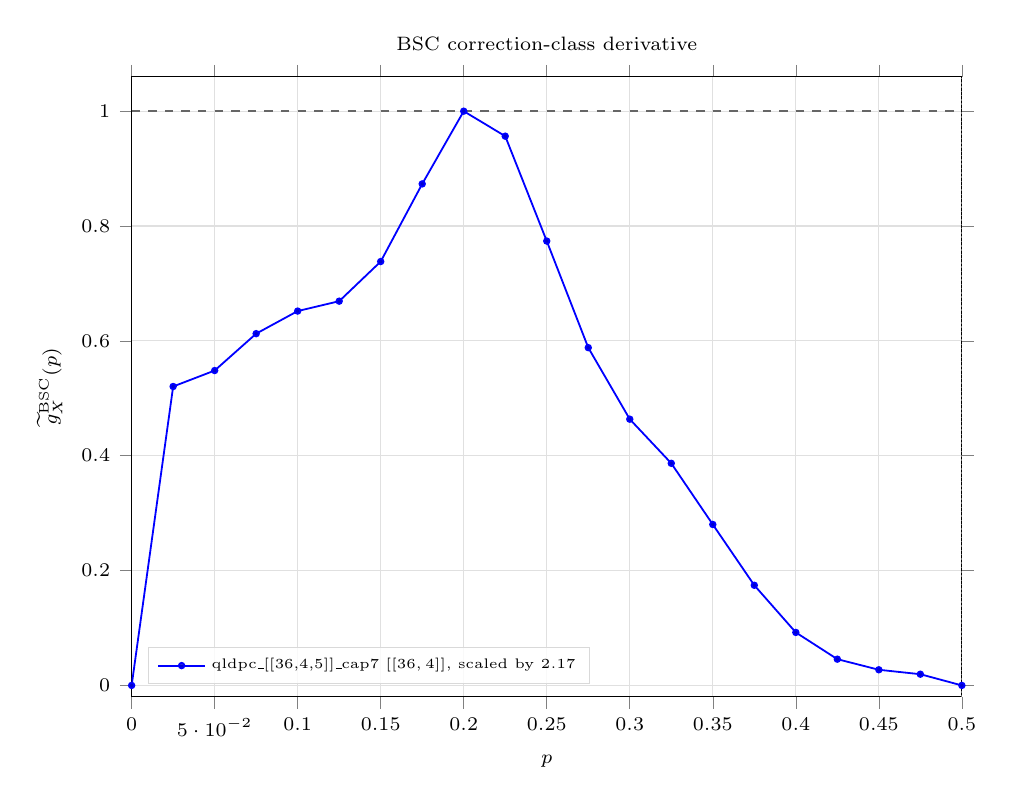
\begin{tikzpicture}
\begin{axis}[
  name=scaledBSCGEXITQldpc3645Cap7Axis,
  width=\linewidth,
  height=0.78\linewidth,
  title={BSC correction-class derivative},
  title style={font=\scriptsize},
  xlabel={$p$},
  ylabel={$\widetilde g_X^{\rm BSC}(p)$},
  xmin=0, xmax=0.5,
  ymin=-0.02, ymax=1.06,
  grid=both,
  major grid style={black!12},
  minor grid style={black!6},
  tick align=outside,
  tick label style={font=\scriptsize},
  label style={font=\scriptsize},
  legend cell align={left},
  legend style={draw=black!15, fill=white, fill opacity=0.82, text opacity=1, at={(0.02,0.02)}, anchor=south west, font=\tiny},
]
\addplot[black!60, densely dotted, line width=0.55pt, forget plot] coordinates {(0.5,-0.02) (0.5,1.06)};
\addplot[black!60, dashed, line width=0.55pt, forget plot] coordinates {(0,1) (0.5,1)};
\addplot+[color=blue, mark=*, mark size=1.0pt, line width=0.65pt]
coordinates {(0,0) (0.025,0.520558795063) (0.05,0.548335399479) (0.075,0.612583377648) (0.1,0.651911420615) (0.125,0.669143354812) (0.15,0.738161627922) (0.175,0.873367771923) (0.2,1) (0.225,0.956471953735) (0.25,0.773831453023) (0.275,0.588192044778) (0.3,0.463633288079) (0.325,0.386772883666) (0.35,0.280289958219) (0.375,0.174403593122) (0.4,0.0922806418289) (0.425,0.0457127834351) (0.45,0.0272564206926) (0.475,0.01951600106) (0.5,0)};
\addlegendentry{qldpc\_[[36,4,5]]\_cap7 $[[36,4]]$, scaled by $2.17$}
\end{axis}
\end{tikzpicture}
